\documentclass{article}

\usepackage[latin1]{inputenc}
\usepackage{tikz}
\usetikzlibrary{calc}
\usepackage{tkz-euclide}
\tikzset{line/.style={draw, thick, -latex'}}
%\usetikzlibrary{shapes,arrows}
\begin{document}
\pagestyle{empty}


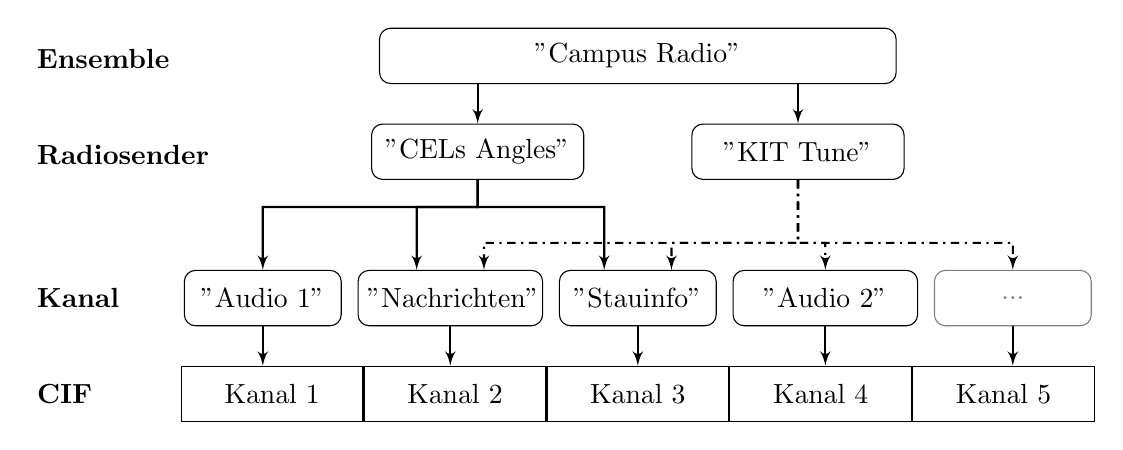
\begin{tikzpicture}[node distance = 1cm, auto]
\tikzstyle{block} = [rectangle, rounded corners, draw, text width=6em, text centered, minimum height=2em]
\tikzstyle{rect} = [rectangle, draw, text width=5.9em, text centered, minimum height=2em]
\tikzstyle{input} = [rectangle, text width=2em, align=right, minimum height=2em]

\node [block, text width=18em](ensemble){"Campus Radio"};
\node [block, below=0.5cm of ensemble.190, anchor=north, text width=7em](sender1){"CELs Angles"};
\node [block, below=0.5cm of ensemble.350, text width=7em](sender2){"KIT Tune"};
\node [block, text width=5em, below=1.5cm of $(sender2.west)!0.5!(sender1.east)$](traffic){"Stauinfo"};
\node [block, left=2mm of traffic](news){"Nachrichten"};
\node [block, text width=5em, left=2mm of news](audio1){"Audio 1"};
\node [block, right=2mm of traffic](audio2){"Audio 2"};
\node [block, right=2mm of audio2, opacity=0.5, text width=5em](etc){...};
\node [rect, below=0.5cm of traffic.south](cif_mid){Kanal 3};
\node [rect, left=0.0cm of cif_mid.west](cif_-1){Kanal 2};
\node [rect, left=0.0cm of cif_-1.west](cif_-2){Kanal 1};
\node [rect, right=0.0cm of cif_mid.east](cif_+1){Kanal 4};
\node [rect, right=0.0cm of cif_+1.east](cif_+2){Kanal 5};
\node [input, left= of cif_-2.west](cif){\textbf{CIF}};
\node [input, above=0.5cm of cif](kanal){\textbf{Kanal}};
\node [input, above=1.1cm of kanal](sender){\textbf{Radiosender}};
\node [input, above=0.5cm of sender](ensemble_label){\textbf{Ensemble}};

\path [line] (ensemble.190) -- (sender1.north);
\path [line] (ensemble.350) -- (sender2.north);
\path [line] (sender1.south) -- ($(sender1.south)!0.3!(news.north-|sender1.north)$) -| (news.140);
\path [line] (sender1.south) -- ($(sender1.south)!0.3!(news.north-|sender1.north)$) -| (audio1.north);
\path [line] (sender1.south) -- ($(sender1.south)!0.3!(news.north-|sender1.north)$) -| (traffic.140);
\path [line, dash dot] (sender2.south) -- ($(sender2.south)!0.7!(audio2.north-|sender2.north)$) -| (audio2.north);
\path [line, dash dot] (sender2.south) -- ($(sender2.south)!0.7!(audio2.north-|sender2.north)$) -| (traffic.40);
\path [line, dash dot] (sender2.south) -- ($(sender2.south)!0.7!(audio2.north-|sender2.north)$) -| (etc.north);
\path [line, dash dot] (sender2.south) -- ($(sender2.south)!0.7!(audio2.north-|sender2.north)$) -| (news.40);
\path [line] (audio1.south) -- (cif_-2.north-|audio1.south);
\path [line] (news.south) -- (cif_-1.north-|news.south);
\path [line] (traffic.south) -- (cif_mid.north-|traffic.south);
\path [line] (audio2.south) -- (cif_+1.north-|audio2.south);
\path [line] (etc.south) -- (cif_+2.north-|etc.south);

\end{tikzpicture}
\end{document}